\documentclass{article}
\usepackage{graphicx}
\usepackage[margin=1.5cm]{geometry}
\usepackage{amsmath}

\begin{document}

\title{Tuesday Reading Assessment: Chapters 4-5}
\author{Prof. Jordan C. Hanson}

\maketitle

\begin{figure}[ht]
\centering
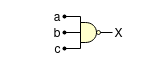
\includegraphics[width=0.2\textwidth]{figures/3_nand.png}
\caption{\label{fig:1} A 3-input NAND gate is LOW only when all three inputs are HIGH.}
\end{figure}

\section{Gray Code Conversion (Review)}

\begin{enumerate}
\item Convert the following bit sequences from binary to gray code: (a) 00 (b) 01 (c) 10 (d) 11 \\ \vspace{1cm}
\item Convert the following bit sequencies from gray to binary code: (a) 00 (b) 01 (c) 11 (d) 10 \\ \vspace{1cm}
\end{enumerate}

\section{Logic Circuits, Boolean Algebra, and Karnaugh Maps}

\begin{enumerate}
\item Consider the three input NAND gate in Fig. \ref{fig:1}.  (a) Based on Fig. \ref{fig:1}, create the truth table for the 3 input NAND.  How many terms would there be in the S-SOP expression for this circuit?  (b) From the data in the truth table, create the 3-variable Karnaugh map. (c) Generate the simplified Boolean expression from the Karnaugh map.  \textit{Hint: remember that cells in the top row are adjacent to those in the bottom row.} \\ \vspace{4cm}
\item Draw a gate or circuit that represents the output of the simplified circuit from the previous exercise.
\end{enumerate}

\end{document}
